\section{Dispositivo experimental}\label{sec:dispositivo-experimental}

El esquema del montaje se muestra en la figura~\ref{fig:montaje}.

\begin{figure}[tbh!]
    \begin{center}
        \begin{tikzpicture}

            \draw[thick, black] (0,4) -- (4,4) node[anchor=south]{$I$};

            \draw[rounded corners] (1, 3) rectangle (3, 3.5);
            \draw[thick,black,-stealth](2,3.25) -- ++(0.75,0);
            \draw[thick,black,-stealth](2,3.25) -- ++(-0.75,0);
            \node at (3.6,3.25) {\footnotesize{Br�jula}};

            \draw (0.5,1) rectangle (3.5,3);

            \draw (2,1.2) ellipse (1.5 and 0.2);
            \draw (2,1.6) ellipse (1.5 and 0.2);
            \draw (2,2) ellipse (1.5 and 0.2);
            \draw (2,2.4) ellipse (1.5 and 0.2);
            \draw (2,2.8) ellipse (1.5 and 0.2);

            \node at (4.1,2) {\footnotesize{Discos}};

            \draw[dashed] (2,4) -- ++(0,-0.75);
            \node at (2.25,3.75) {\footnotesize{$d$}};

        \end{tikzpicture}
        \caption{Br�jula bajo el hilo conductor sobre una pila de discos.}
        \label{fig:montaje}
    \end{center}
\end{figure}

Consiste en un cable conductor, r�gido y rectil�neo, por el que circula una corriente $I$,
colocado horizontalmente sobre una br�jula, que a su vez est� apilada sobre una serie de discos, lo
que nos permite variar la distancia $d$ entre la br�jula y el cable.

El campo magn�tico generado $B$ est� contenido en el plano horizontal y es perpendicular al cable.
Si se alinea la direcci�n del cable con la br�jula cuando no circula corriente $I$, tenemos la situaci�n reflejada en
la figura~\ref{fig:vectores}, vista desde arriba del dispositivo.


\begin{figure}[tbh!]
    \begin{center}
        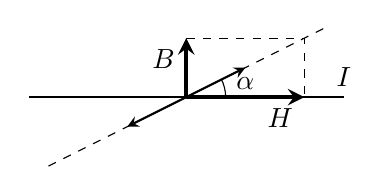
\begin{tikzpicture}

            \draw[thick, black] (0,0) -- (4,0) node[anchor=south]{$I$};

            \draw[ultra thick,black,-stealth](2,0) -- ++(1.5,0) node[anchor=north east]{$H$};
            \draw[ultra thick,black,-stealth](2,0) -- ++(0,0.75) node[anchor=north east]{$B$};

            \draw[dashed] (2,0.75) -- ++(1.5,0) -- ++(0,-0.75);
            \draw[dashed] (0.25,-0.875) -- ++(3.5,1.75);
            \draw[thick,black,-stealth](2,0) -- ++(0.75,0.375);
            \draw[thick,black,-stealth](2,0) -- ++(-0.75,-0.375);

            \draw (2.5,0) arc (0:28:0.5);
            \node at (2.75,0.175) {$\alpha$};

        \end{tikzpicture}
        \caption{Componente horizontal $H$ del campo magn�tico terrestre, campo $B$ inducido por la corriente y �ngulo $\alpha$ entre la
        br�jula y el hilo conductor.}
        \label{fig:vectores}
    \end{center}
\end{figure}

En esta situaci�n, el campo magn�tico generado $B$ y la componente horizontal del campo magn�tico terrestre $H$ son perpendiculares,
y la aguja de la br�jula se desv�a un �ngulo $\alpha$ tal que:

\begin{equation*}
    \tan{\alpha} = \frac{B}{H}
\end{equation*}

Sustituyendo el valor de B dado por la ecuaci�n~\ref{eq:campo}, tenemos:

\begin{equation}
    \tan{\alpha} = \frac{\mu_0}{2\pi d H} \, I
\end{equation}

